\subsection{Fator $\gamma$ do ar: Método de Clément – Desormes}

Nesse experimento, para a determinação do fator $\gamma$ do gás, utilizaremos um dispositivo composto por uma grande garrafa de vidro – contendo ar – que conta com um tampão que pode ser aberto e fechado. Acoplaremos a essa garrafa, um manômetro de coluna de água que ficará aberto. Utilizaremos também, uma bomba manual ligada à garrafa, para a pressurização do gás ali presente.

\begin{figure}[H]
  \centering
  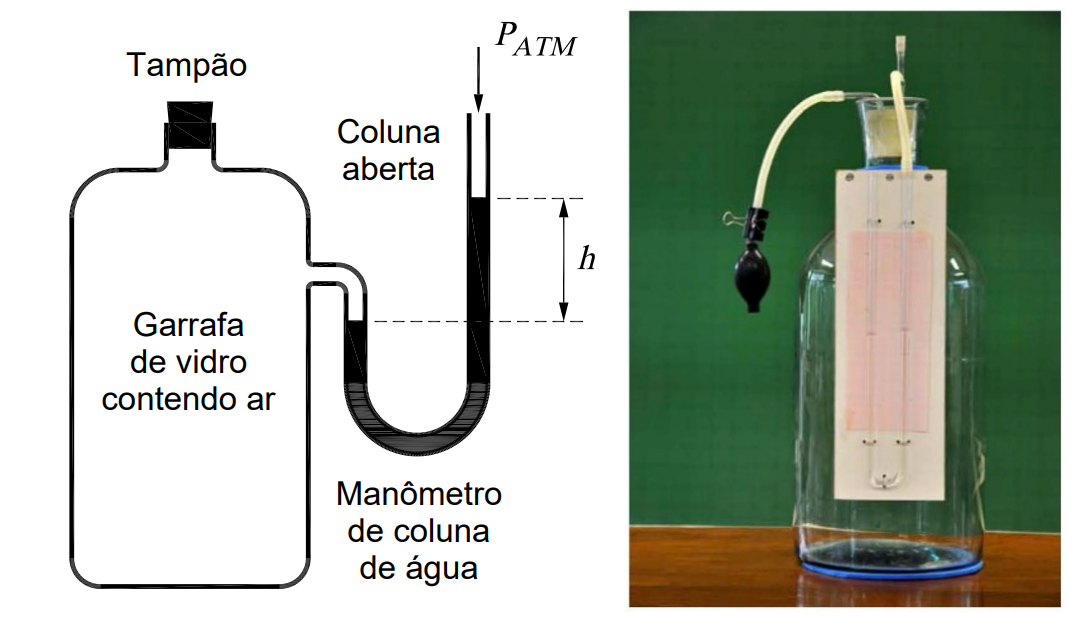
\includegraphics[scale=0.67]{images/Método Clément-Desormes.png}
  \caption{Esquema do dispositivo com o manômetro acoplado e a montagem experimental Clément-Desormes.}
\end{figure}

Vamos procurar a medida do calor específico de um gás – no caso, o ar atmosférico. Para isso, o recipiente rígido descrito acima – o qual permite pouca expansão térmica dentro da faixa de temperatura analisada –, será muito útil. Assim, o valor a ser medido será o calor específico a volume constante $c_V$. Sabemos que o valor $c_P$ – calor específico medido à pressão constante – de um gás é maior que $c_V$, já que no experimento, à pressão constante, o calor cedido ao conjunto também é usado para expandir o gás, mostrando que parte da energia foi transformada em trabalho (expansão) e não apenas em aumento da energia térmica do corpo em questão (aquecimento).\\

A razão entre as capacidades térmicas à pressão e volume constante é o valor do coeficiente $\gamma$ que estamos buscando, um número que aparece muitas vezes nas descrições de processos termodinâmicos gasosos. Podemos também, medir essa razão por meio de processos isobáricos e isocóricos, calculando o calor específico à pressão ($c_P$) e volume constante ($c_V$), respectivamente. Esse experimento foi realizado pelos químicos Nicolas Clément e Charles-Bernard Desormes, pioneiramente, em 1819 – por conta disso, o a técnica utilizada por nós nesse experimento recebe o nome desses cientistas. \\

O método criado por esses estudiosos consiste em aplicar sobre o gás – o qual consideraremos como um gás ideal – dois processos, que serão mostrados na figura a seguir: uma expansão adiabática do estado (1) até o (2), e um aquecimento isocórico de (2) até (3).\\

\begin{figure}[H]
  \centering
  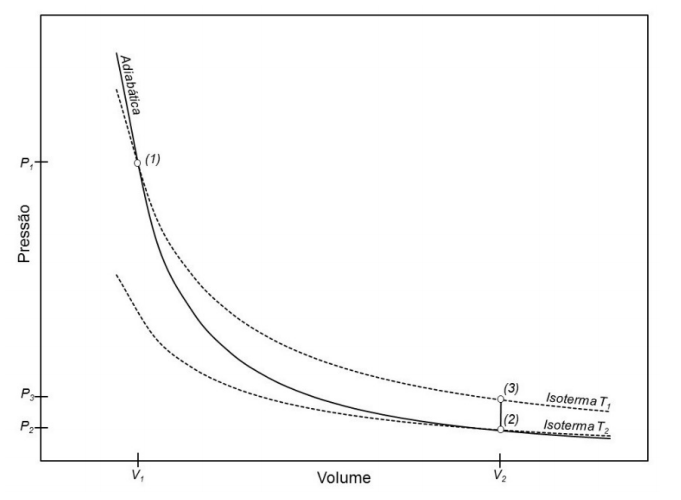
\includegraphics[scale=1]{images/Diagrama PV.png}
  \caption{Diagrama $P-V$ para o processo aplicado sobre o ar, no experimento de Clément – Desormes.}
  \label{fig:processo-grafico}
\end{figure}

No estado inicial de equilíbrio (1), um número $n$ de mols de gás estão à pressão $P_1$ – acima da pressão atmosférica –, com um volume $V_1$ e uma temperatura inicial $T_1$ – igual à temperatura ambiente. Fazemos uma expansão adiabática até o estado (2) com uma pressão $T_2$ - igual à pressão atmosférica –, volume $V_2$ e uma temperatura $T_2$ – menor que a temperatura ambiente. Então, realizamos um aquecimento isocórico do estado (2) até o estado (3), à temperatura ambiente $T_1$ e pressão $T_3$.
O coeficiente $\gamma$ do gás pode ser conseguido tendo em vista a relação entre $P$ e $V$ durante um processo adiabático. Como $PV^\gamma$ constante, podemos dizer que:

\[ P_1V_1^\gamma =  P_2V_2^\gamma\]\

\ Dessa relação, é possível chegar a escrever o fator $\gamma$ como:

\[ \gamma = \frac{ln\frac{P_2}{P_1}}{ln\frac{V_1}{V_2}}\]\

\ Buscando facilitar nossos cálculos, seria ideal que conseguíssemos expressar $\gamma$ somente em termos das pressões, que conseguimos encontrar mais facilmente em nosso modelo experimental. Para calcular o coeficiente $\gamma$ apenas em função das pressões – não dependendo dos volumes, visto que na prática seria difícil medi-los com precisão – podemos observar o processo isocórico entre o ponto (2) e o ponto (3). Como os estados (1) e (3) estão sobre a mesma curva isoterma, sabemos que a temperatura em (3) é idêntica à de (1), ou seja, $T_1$. Logo:

\[ \gamma = \frac{ln\frac{P_2}{P_1}}{ln\frac{P_3}{P_1}}\] \

\ Nesse experimento, usaremos o valor das pressões para calcular o fator $\gamma$ assim, precisaremos determinar as diferentes pressões envolvidas no problema. Para isso, usaremos um manômetro de coluna de água aberto em uma das extremidades – já supracitado.\\

Poderemos achar as pressões em função da altura h da coluna de água, da seguinte maneira:

\[ P_1 = P_{atm} + \rho g h_1 \]
\[ P_2 = P_{atm} \]
\[ P_3 = P_{atm} + \rho g h_3 \] \


\ Como $P_2$ é igual à pressão atmosférica $P_{atm}$, sua altura $h_2$ da coluna de água deve ser nula ($h_2 = 0 $). Dessa forma, utilizando a equação deduzida acima para $\gamma$ podemos calcular esse fator a partir de $P_{atm}$, $h_1$ e $h_3$.\\

As pressões $P_1$ e $P_3$ podem ser reescritas como:

\[ P_1 = P_{atm} ( 1 + \frac{\rho g h_1}{P_{atm}}) \ \ \  e \ \ \   P_3 = P_{atm} ( 1 + \frac{\rho g h_3}{P_{atm}})   \] \
 
\ Usando uma expressão logarítmica, apresentada como uma série infinita:

\[ ln(1 + x) = x - \frac{x^2}{2} + \frac{x^3}{3} - \frac{x^4}{4} + ...  \]\ 
 
\ Podemos tomar uma aproximação válida para essa série, quando x<<1, que consiste em perceber que o termo que importa é somente o primeiro (x), visto que os demais, por serem muito pequenos, tendem a zero e pouco influenciam no resultado final. Então, concluímos que:
\[ ln(1 + x) \approx x \] \

\ Juntando as expressões já encontradas por nós, teremos:

\[ \gamma = \frac{h_1}{h_1 - h_3} \] \ 

\ E assim, terminaremos o experimento, descobrindo o fator gama do ar pelo método de Clément-Desormes, baseando-se apenas nas alturas $h_1$ e $h_3$ dadas no manômetro.
